\documentclass[11pt]{article}

\usepackage[paper=a4paper,left=25mm,right=25mm,top=25mm,bottom=25mm]{geometry}
\usepackage{url}
\usepackage{notoccite}
\usepackage{graphicx}
\usepackage{multirow}
\usepackage{verbatim}
\graphicspath{ {images/} }

%opening
\title{Cloud Computing Project - Analyzing the connection between flights and cases of Covid-19 in Europe: Report}
\author{Aeilko Lübsen}

\begin{document}
	
	\maketitle
	
	The epidemiological measures to contain the coronavirus outbreak in 2020 had an impact on international air traffic. This project is about developing a system, which analyzes the connection of cases of Covid-19 and air traffic based on datasets containing Covid case and flight data in Europe. It uses publicly available datasets of flights, airports, regional Covid-19-cases and the geographical make-up of these regions \cite{airtraffic2021, covid2022, nuts2016, airports2022}. The project uses a microservice architecture implemented in Python, which communicates using GRPCs. Because the datasets contain geo-spatial data the system is backed by a PostGIS database. The functionalities of these microservices are then exposed through an API that is supposed to support a frontend, which was not implemented as it goes beyond the scope of this project.
	
	\section{Motivation and Dataset Characterization}
	
	The motivation for this project is the simple hypothesis that there is an influence on air traffic caused by the number of Covid-19 cases, because there were political measures implemented to ban or at least add significant obstacles to international travel. I wanted to create a backend supporting a heatmap of flights and Covid cases that can also display some deeper data analysis to illuminate this connection for single airports and their surrounding areas.
	
	To do this, I firstly chose two datasets containing information on the number of flights over the course of the pandemic and regional data on Covid-19 cases in the EU. To be able to link these, I also used a dataset provided by Eurostat that has the geo-spatial information of the regions that the Covid-19 dataset contains and another one that contains the locations of airports. Combining these datasets, we can first join the flight data with the airports, which can be joined with the regions that the airports are in, which can then be joined with the Covid cases, which in turn yields the required relationship between flights and Covid cases. A visual explanation of this can be seen in Figure~\ref{fig:datasets}.
	
	\begin{figure}[h!]
		\centering
		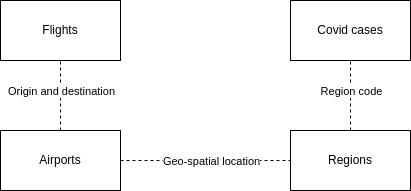
\includegraphics[scale=0.6]{datasets.png}
		\caption{A visualization of the connection between the datasets.}
		\label{fig:datasets}
	\end{figure}

	\subsection{Flights}
	
	The flights dataset contains most importantly the origin and destination airport as well as the time the flight was first and last seen (which is an estimate for departure and arrival times). On top of this, there is the flight's callsign, commercial number, transponder identifier, the aircraft tail number and aircraft model.
	
	\subsection{Airports}
	
	The airports dataset contains an ID, the 4-letter ICAO airport code (which matches with the code used in the flights datasets for origin and destination), the size of the airport, the geolocation and continent and some additional info which is irrelevant to our use cases like the airport's elevation and Wikipedia link.
	
	\subsection{Covid Cases}
	
	The Covid case dataset contains the 14-day incidence of Covid cases per 100,000 inhabitants of each region per day. So for every day since the start of the pandemic it has the date, country and region name, a region code, the incidence and the source of the data, because it is accumulated from different institutes all over Europe.
	
	\subsection{Regions}
	
	The regions dataset is the standard partition of the EU by Eurostat in three sub-levels called NUTS. It has the same region code used in the Covid case dataset and a geo-spatial geometry that describes the boundaries of these regions.
	
	\section{Use Cases and REST API}
	
	As explained above, the system is supposed to support a frontend, which shows a heatmap displaying the number of Covid cases and flights on a certain date. With a slider this date can be modified to show the temporal change of these statistics. On this map, single airports could be selected to see diagrams on the number of flights and Covid cases over time more specifically as well as some statistical analysis on these data. Additionally, it could show the change in flights compared to the time before the pandemic. To survey the runtime performance, an administrator can also request the average runtime of certain GRPC requests. The use case diagram is shown in Figure~\ref{fig:use_cases}.
	
	\begin{figure}[h!]
		\centering
		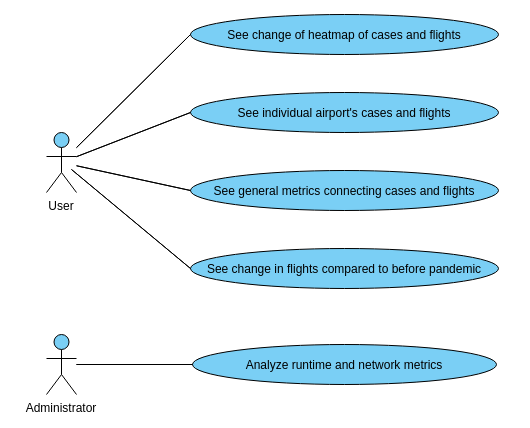
\includegraphics[scale=0.6]{use_cases.png}
		\caption{Use case diagram for the system.}
		\label{fig:use_cases}
	\end{figure}

	The REST API to support these use cases has five endpoints to support these use cases. Firstly, the aforementioned administrator endpoint that returns the average runtime of certain GRPC requests. For the heatmap, there is an endpoint that returns the location of all airports and the number of Covid cases in an airport's area over time. Additionally, there is an endpoint returning the number of Covid cases in every region on a certain date and the number of flights on each route on a certain date. Then there is one endpoint that calculates a statistic linking covid cases and flights for a certain airport's area together. An overview over all existing endpoints can be seen in Table~\ref{tab:endpoints}.
	
	\begin{table}
	\begin{center}
	\begin{tabular}{|c|c|}
		\hline
		Path & Description \\
		\hline
		\texttt{/airports} & location and name of all airports \\
		\hline
		\texttt{/covid\_cases} & number of Covid cases in all regions on a certain date \\
		\hline
		\texttt{/flights} & number of flights on all connections on a certain date \\
		\hline
		\texttt{/airport\_covid\_cases} & number of Covid cases in an airport's area over time \\
		\hline
		\texttt{/airport\_statistics} & statistic linking covid cases and flights in an airport's area \\
		\hline
		\texttt{/runtimes} & the average runtime of a certain GRPC request \\
		\hline
	\end{tabular}
	\end{center}
	\caption{All endpoints in the REST API}
	\label{tab:endpoints}
	\end{table}


	\section{Architecture}
	
	Figure~\ref{fig:architecture} shows an overview over the microservice architecture for the system. It only exposes a single API to the outside user, which is optimized to be used by a specific frontend. Behind this API are four different microservices. Two of the microservices directly concern the data from the datasets. The data delivery service reads flight and case data from the database and forwards it to the API, while the data analysis microservice performs statistical operations to gain deeper insights into the gathered data. The data required for these operations is exclusively gathered from the data delivery microservice, so as to minimize the number of microservices that have to directly interact with the database. Both of these services also write their runtimes into the database, so the administrator analysis microservice can analyze and pass it to the outbound API. Also, the architecture implements the central logging pattern, therefore there is a separate logging microservice. As a database management system, I chose to use PostGIS to best support the required geographical operations. This database was filled automatically by an ingestion pipeline that downloads the datasets from the web, parses the files and inserts the data.
	
	\begin{figure}[h!]
		\centering
		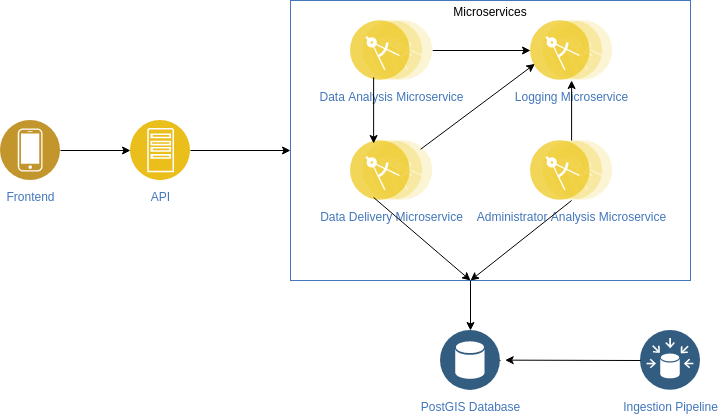
\includegraphics[scale=0.38]{architecture.png}
		\caption{Preliminary architecture for the system.}
		\label{fig:architecture}
	\end{figure}

	\section{Implementation}
	
	The implementation of the project can be separated into three phases. At first, the ingestion pipeline had to be realized, so the microservices could be implemented. After this was done, the project was revised and reworked.
	
	\subsection{Ingestion}
	
	The implementation of the ingestion pipeline seemed at first to be rather straight-forward. All datasets needed to be downloaded and then the required columns of the data had to be inserted into the correct tables row by row. For the smaller datasets containing the regions, airports and Covid cases this approach worked pretty well. The only problem I encountered was converting the geographical data to the correct hexadecimal format. However, this simple approach took multiple days to finish for the flight dataset, because it was too big. The dataset split up into monthly batches zipped by themselves added some more complexity. Instead, each file had to be imported by itself with the PSQL copy command before it could be selected into the final table only containing the necessary data. Additionally, I took only a sample of about 10\% of the data, because otherwise the more complex queries required for the running program would have runtimes longer than a minute. Additionally, I removed some of the unnecessary columns like the coordinates at which the flights were first and last seen.
	
	\subsection{Microservices}
	
	In the first step, only three of the microservices were implemented, while the logging microservice was only added in the revision of the project. Each microservice is configured by a .env-file that contains the addresses of all other required microservices and the database credentials. I will describe their implementation in chronological order.
	
	\subsubsection{Data Delivery}
	
	The data delivery microservice as the most basic microservice just accessing data from the database has five remote procedures it implements: 
	
	\begin{itemize}
		\setlength\itemsep{0em}
		\item \texttt{Airports} - returning the names and locations of all airports (optionally filtered by continent and size)
		\item \texttt{Flights} - returning the number of flights on each connection (filtered by date and optionally by continent of origin or destination)
		\item \texttt{FlightsByDate} - returning the number of flights on each connection for a single airport on each day (filtered by either origin or destination airport)
		\item \texttt{CovidCases} - returning the number of Covid cases in each region (fitered by date)
		\item \texttt{AirportCovidCases} - returning the number of Covid cases in the region around an airport over time
	\end{itemize}

	The actual GRPC service contains an additional class, a database service that performs all the database queries, of which it just calls the respective function and then packages it into the GRPC response object and returns it. The main challenge in the implementation of this microservice was figuring out how to work in the general GRPC framework, trying to figure out how to address the other services and getting how to deal with the automatically generated class files, also for deployment later.
	
	\subsubsection{Data Analysis}
	
	The data analysis microservice has only one remote procedure called \texttt{AirportAnalysis}. It returns a statistical analysis of the influence of rising Covid-19 cases in the surrounding area of an airport on air traffic. To do this, it first determines the maximum Covid-19 incidence reached in the region. Then it normalizes all incidences with this maximum. Next, it collects the relative number of flights on a day in 2020 compared to the same day in 2019 before the pandemic. This is multiplied with the normalized coronavirus incidence on that day. This is performed for each day in 2020, where the incidence was greater than zero and there was at least one flight. I named this statistic, the Covid-flight-factor. If it is higher, it generally means that there was a high incidence and/or a big change in flights to the year before. All the data used in this operation is requested from the data delivery microservice.
	
	\subsubsection{Administrator Analysis}
	
	The administrator analysis microservice offers a single remote procedure called \texttt{RequestAnalysis} that gets the GRPC service and request as a parameter as well as a time frame. It will then get the average runtime of all executions of the specified request over the course of this time frame from the database. The more interesting part of this functionality lays not in the microservice itself, but in how this data is inserted into the table. To do this, I created a GRPC interceptor that is added to both the data delivery and data analysis service classes. This interceptor contains a function that is called on each remote procedure call. This function first saves the time of the beginning of the call and then adds a callback to the GRPC context, which is called when the GRPC returns. In this callback, the starting time is subtracted from the finishing time to determine the runtime and then inserted into the database.
	
	\subsubsection{Logging}
	
	The logging microservice was implemented in the revision of the project. It offers a single remote procedure simply called \texttt{Log}. It has three parameters, the message, the origin microservice and the log level. On receiving the call the message is written both into a central log and into a single log that is being kept for each single microservice. Once again, the more interesting work of this microservice was in how to redirect the \texttt{stdout} of the other microservices to automatically write the \texttt{print} output directly to this central log. To do this, I implemented a class called \texttt{LoggingRedirector}, which saves the original \texttt{stdout} and has a \texttt{write} method. When it is set as the system \texttt{stdout} this method is called and it sends a GRPC to the logging microservice, while also printing the output to the original \texttt{stdout}.
	
	\subsection{Outbound}
	
	The outbound API is implemented as a simple Flask app. With the help of the package \texttt{connexion} the OpenAPI specification is directly used to minimize the required work and avoid any errors in setting up the correct paths. All it then needs to do is creating clients to the data analysis, data delivery and administrator analysis microservices and perform the request that is required to return a response, because every API call that is specified, directly maps to one of the remote procedures of the microservices.
	
	\section{Deployment}
	
	When it came to the deployment of this system, I encountered a lot of different problems. I got it to run on my local minikube instance with a deployment with a single replica for each service, all of the deployments having a service to be connected to each other. The first problem that I encountered after this, was getting the local Docker images to an online cloud registry. I first tried to use GitHub Actions to build the images, when a commit to the git repository happens and then push them to the Google Cloud Artifact Registry. For a reason I can still not determine at this point, the second part - pushing to the repository - would always fail and retry until the GitHub Action timed out. Next, I tried pushing my local images to the Google Cloud Registry, which would also fail with a hard to understand error message. After hours of trying to fix the problem, I reinstalled Docker on my machine and the error disappeared and I could finally push to the Artifact Registry. The next problem was, that I could not figure out how to address the different services inside the cluster independently of their actual IP. This process was complicated by the fact that I did not 
	
	\section{Tests and Evaluation}
	
	When it comes to tests, I only implemented unit tests for all four microservice classes. They all pass. I failed to implement integration tests and also did not measure any further metrics.
	
	\section{Conclusion}
	
	In this project, I implemented a functioning microservice architecture of a backend for a webapp. This app was deployed to a kubernetes cluster and unit-tested on my local machine. However, some of the goals for this project could not be reached. For once, the deployment to the cloud did not work and there are no further tests or evaluations that were performed beyond the unit tests. The main reason for this was the fact that I had to work on this project alone, which for one meant I could not split up the workload between multiple people, but I believe even more crucially, it meant that I could not discuss my problems with the deployment and let somebody else test my code and see if it worked for them. I think, this project had the potential to be a lot bigger and more interesting, because the choice of datasets would have allowed a more thorough and deep analysis of the matter. It would also have been interesting to actually build a front-end and optimize the code for this application. Despite its shortcomings, I would still rate this project a success, because it gave me a lot of skills I would consider vital for my future career in software engineering.
	
	\newpage
	
	\bibliographystyle{unsrt}
	
	\bibliography{references.bib}
	
\end{document}